\chapter{Kompontentendesign}
\label{chap:komponentendesign}

\begin{figure}
    \label{figure:diagrammanordnungsverfahren}
    \begin{center}
    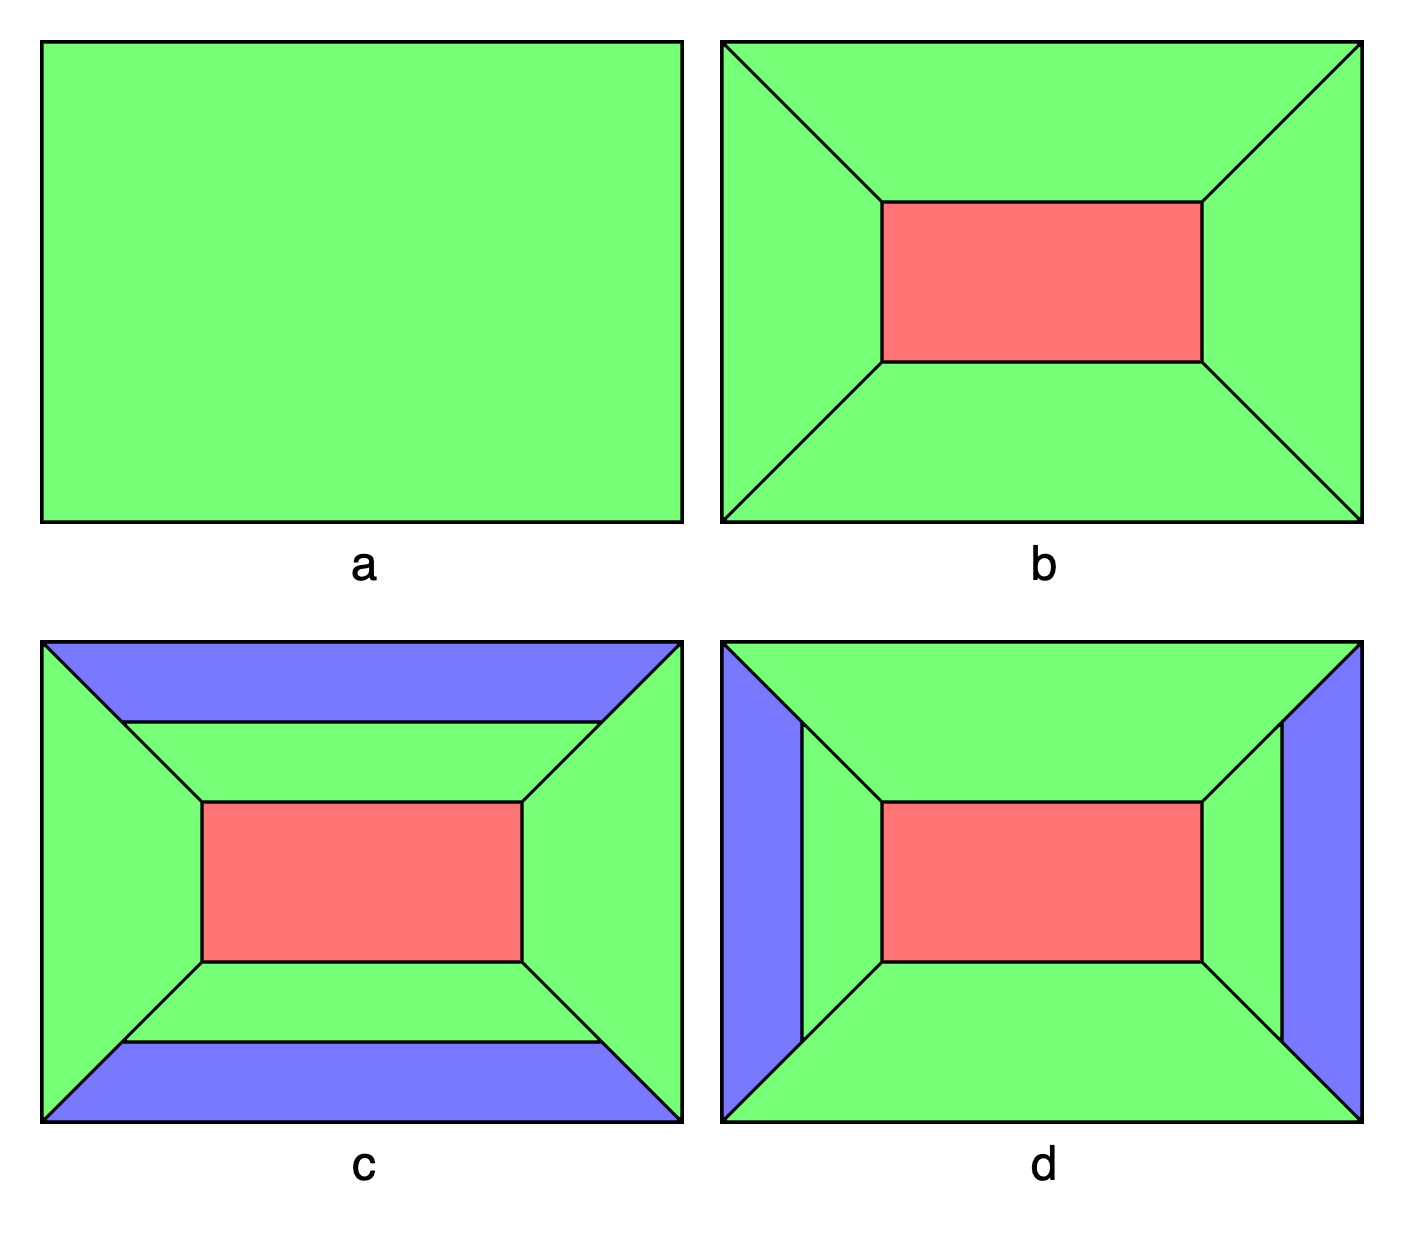
\includegraphics[scale=0.2]{img/abbildungen/Diagrammanordnunsverfahren}
    \end{center}
    \caption{Diagrammanordnunsverfahren}
\end{figure}



\section{Trennung von Logic}
\label{sec:trennungvonlogic}
% Reduzierung von Abhängigkeiten,
% Gemeinsamkeiten wischen mehreren services? beispiel API und Delivery
% Eigene Datenbanken etc
% Separation of Concerns, etwa Trennung der Zuständigkeiten


\subsection{Microfrontend}
\label{subsec:Microfrontend}
Domain Driven Development also in Frontend.

Aufteilung in Module, die während der laufzeit geladen werden.
Seite 171 in Buch (Eberhard Wolff Microservices) befasst sich mit dem
Thema, wenn auch nicht auf das dynamische Laden eingegangen wird.
"Das Deployment der SPA ist meistens nur als vollständige Anwendung möglich."
Neuer Ansatz für unabhängiges Deployment!

-> Auch Problem: Deployment Monolith -> Separation der Deployment Vorgänge

-> "Wenn in einem Microservice ein Feature umgesetzt wird, das auch Änderungen
in der Client-Anwendung benötigt, kann diese Änderung nicht durch eine neue
Version des Microservice alleine ausgerollt werden. Es muss auch eine neue Version
der Client-Anwendung ausgeliefert werden." Seite 176.  (Eberhard Wolff Microservices)
Absatz 3.

Deployment abhängigkeiten verringern!

SOAP Schnittstelle zwischen Frontend Chart Plugins und Frontend Arrangement Software!
Weniger bis garkeine Abhängigkeit von Implementierungsdetails

Problem: Steigende Komplexität der Anwendung.

\subsection{Microbackend}
\label{subsec:microbackend}

\section{Protokolle}
\label{sec:protokolle}
% Also question ? Send batches which server can immediately handle
% or does the server has to wait till all the data has arrived
\subsection{HTTP 2}
\label{subsec:http2}

\subsection{Websockets}
\label{subsec:websockets}

% Cite this text: Another useful feature of being able to establish a connection using
% HTTP is the ability to use HTTP authentication semantics for the socket,
% such as the Authorization header for Basic Auth or Bearer Token Auth.
% https://codeburst.io/why-you-don-t-need-socket-io-6848f1c871cd

\section{Schnittstellengestaltung}
\label{sec:schnittstellengestaltung}

\subsection{Open API 3.0}
\label{subsec:openapi3}

\subsection{AsyncAPI}
\label{subsec:asyncapi}

\subsection{GraphQL Subscriptions}
\label{subsec:graphqlsubscriptions}

\section{Sicherheit}
\label{sec:sicherheit}

\subsection{Middlewares}
\label{subsec:middlewares}

\subsection{JWT}
\label{subsec:jwt}
% JWT vs Session
% Whitelist statt Blacklist

\section{Skalierbarkeit}
\label{sec:skalierbarkeit}
